\documentclass{paper}

%\usepackage{times}
\usepackage{epsfig}
\usepackage{graphicx}
\usepackage{amsmath}
\usepackage{amssymb}
\usepackage{color}
\usepackage{subcaption}
\usepackage{caption}


% load package with ``framed'' and ``numbered'' option.
%\usepackage[framed,numbered,autolinebreaks,useliterate]{mcode}

% something NOT relevant to the usage of the package.
\setlength{\parindent}{0pt}
\setlength{\parskip}{18pt}






\usepackage[latin1]{inputenc} 
\usepackage[T1]{fontenc} 

\usepackage{listings} 
\lstset{% 
   language=Matlab, 
   basicstyle=\small\ttfamily, 
} 



\title{Report Computer Vision Project 1}



\author{Single Michael\\08-917-445}
% //////////////////////////////////////////////////


\begin{document}



\maketitle


% Add figures:
%\begin{figure}[t]
%%\begin{center}
%\quad\quad   \includegraphics[width=1\linewidth]{ass2}
%%\end{center}
%
%\label{fig:performance}
%\end{figure}

\section{Photometric Stereo (Due on 28/10/2014)}



\paragraph{1. Calibration (35 points)}
In this section you should:

\begin{itemize}
\item Describe the algorithm you used for calculating the light directions given the images of the chrome sphere for different lighting conditions. You need to provide the formula you used to calculate such directions given: 1) The radius of the sphere; 2) The 2D coordinates of the light source highlights on the sphere; 3) The 2D coordinates of the centre of the sphere; 4) The unit vector $(0,0,-1)$ that points towards the camera.
\item The calculated light vector in the following format: 
\begin{align}
\mathbf{L}= \left[ \begin{array}{cccccccccccccc}
L_{1x} & L_{2x} & L_{3x} & L_{4x} & L_{5x} & L_{6x} & L_{7x} & L_{8x} & L_{9x} & L_{10x} & L_{11x} & L_{12z}\\
L_{1y} & L_{2y} & L_{3y} & L_{4y} & L_{5y} & L_{6y} & L_{7y} & L_{8y} & L_{9y} & L_{10y} & L_{11y} & L_{12y}\\
L_{1z} & L_{2z} & L_{3z} & L_{4z} & L_{5z} & L_{6z} & L_{7z} & L_{8z} & L_{9z} & L_{10z} & L_{11z} & L_{12z}
\end{array} \right] \nonumber
\end{align}
\end{itemize}

In this section we discuss and derive all essential formulas in order to compute light direction vectors using the technique of photometric stereo. Afterward, we discuss in detail how some quantities, such as the sphere radius, are computed.  \\

We start by describing how normals on a spherical surface can be computed. Next, we discuss how we can compute the surface normals of the images of a chrome sphere. Last, by using Snell's reflection law, we tell the reader how the light directions can be estimated. \\

Every point $(x,y,z)$ on the surface of a sphere in $\mathbb{R}^3$ with a radius $r$ centered at $\textbf{c} = (c_x, c_y, c_y)$ fulfills the following implicit function:
\begin{equation}
    r^2 = (x-c_{x})^2 + (y-c_{y})^2 + (z-c_{z})^2
\label{eq:param_sphere}
\end{equation}

Equation $\ref{eq:param_sphere}$ has the following vectorized representation:

\begin{equation}
    f(\textbf{p}) = (\textbf{p}-\textbf{c}) \cdot (\textbf{p}-\textbf{c}) -r^2 = 0
\label{eq:param_sphere_vec}
\end{equation}

Where $\textbf{p}$ denotes a point $(x,y,z)$ on the sphere's surface. Please note that $f$ denotes the implicit function (for our case the implicit function of a sphere). An implicit function describes a set of surface points whenever we set this function equal to zero, i.e. $f(p) = 0$. \\

Next we describe how we can compute the normal on a sphere using our implicit representation defined in equation $\ref{eq:param_sphere_vec}$. From Mathematics we know that the normal on a surface point $\textbf{p}$ is simply the gradient of the implicit function describing the surface. Thus, the equation for computing a normal from $f$ looks like:
\begin{equation}
     	\textbf{n}(\textbf{p}) = \nabla f(\textbf{p})
\label{eq:normal_impfunc}
\end{equation}

For simplification purposes we omit the argument $\textbf{p}$ in $\textbf{n}(\textbf{p})$ in the following and just write $\textbf{n}$ instead. \\

Applying the identity from equation $\ref{eq:normal_impfunc}$ to equation $\ref{eq:param_sphere_vec}$ we can compute the normal on the surface of a sphere.

\begin{align}
\textbf{n}
&= \textbf{n}(\textbf{p}) \nonumber \\
&= \nabla f(\textbf{p})  \nonumber \\
&= \nabla \left((\textbf{p}-\textbf{c}) \cdot (\textbf{p}-\textbf{c}) -r^2\right) \nonumber \\
&= 2(\textbf{p}-\textbf{c})
\label{eq:impl_sphere_normal}
\end{align}

Please note that the normal $\textbf{n}$ from equation $\ref{eq:impl_sphere_normal}$ is not 
normalized. The normalized normal $\hat{\textbf{n}}$ of the normal from equation $\ref{eq:impl_sphere_normal}$:

\begin{align}
\hat{\textbf{n}}
&= \frac{\textbf{n}}{||\textbf{n}||} \nonumber \\
&= \frac{(\textbf{p}-\textbf{c})}{r}
\label{eq:impl_sphere_norm_normal}
\end{align}

Therefore, equation $\ref{eq:impl_sphere_norm_normal}$ tells us how we can compute normalized normals at any point lying on the surface of a implicit surface. \\

Next, we describe how we can make use of equation $\ref{eq:impl_sphere_norm_normal}$ when using our twelve images of the chrome sphere. Since the given images are in 2d, i.e. only exhibit two dimensions, the x-and y-coordinate, we cannot make directly use of the z component in order to define the surface of a sphere using its implicit representation from equation $\ref{eq:param_sphere}$. \\

Thus, we express the $z$ component as a parametrization of $(x,y,r)$:

\begin{align}
z 
&= z(x,y,r) \nonumber \\
&= \sqrt{r^2 - (x-c_x)^2 - (y-c_y)^2}
\label{eq:z_comp}
\end{align}

In order to derive this identiy we only solved for $z$ using equation $\ref{eq:impl_sphere_norm_normal}$. By plugging equation $\ref{eq:z_comp}$ into equation \ref{eq:impl_sphere_norm_normal} we get the final representation for computign the normals:

\begin{equation}
    \hat{\textbf{n}} = 
    \frac{1}{r}\left(
        \begin{array}{c}
            (x-c_{x}) \\
            (y-c_{y}) \\
            -\sqrt{r^2 - (x-c_x)^2 - (y-c_y)^2}
        \end{array}
    \right)
\label{eq:final_normal}
\end{equation}

Where $(x,y)$ are coordinates on the chrome sphere exhibiting a (specular) highlight caused by light sources. For any such $(x,y)$ we compute its normal using equation $\ref{eq:final_normal}$. Please note that we are using the negative of z as the third component in the normal vector in $\ref{eq:final_normal}$ since the z-axis points towards the camera eye (our convention).  \\

Last, using all these computed normals, we can estimate the light directions using Snell's reflection law:

\begin{equation}
    L_k = \textbf{d}-2(\textbf{d}\cdot \hat{\textbf{n}}_k)\hat{\textbf{n}}_k
\label{eq:snell_reflection}
\end{equation}

Where $L_k$ denotes the k-th light source resulting from the k-th normal vector $\hat{\textbf{n}}_k$.  \textbf{d} = $(0,0,-1)$ denotes the direction of the camera from any point.\\

All retrieved light directions $L_k$ can be assembled into a matrix $\mathbf{L}$. 

\begin{align}
\mathbf{L}^T= \left[ \begin{array}{ccc}
    0.4979 &  -0.4672 &  -0.7306 \\
    0.2441 &  -0.1376 &  -0.9599 \\
   -0.0386 &  -0.1768 &  -0.9835 \\
   -0.0953 &  -0.4443 &  -0.8908 \\
   -0.3214 &  -0.5095 &  -0.7982 \\
   -0.1114 &  -0.5652 &  -0.8174 \\
    0.2828 &  -0.4257 &  -0.8595 \\
    0.1013 &  -0.4335 &  -0.8954 \\
    0.2073 &  -0.3367 &  -0.9185 \\
    0.0889 &  -0.3344 &  -0.9382 \\
    0.1298 &  -0.0465 &  -0.9904 \\
   -0.1446 &  -0.3644 &  -0.9199
\end{array} \right] \nonumber
\end{align}

$\mathbf{L}^T$ denotes the transposed of the matrix $\mathbf{L}$. \\

I computed $(x,y)$ coordinates the sphere center from the given mask matrix. The same holds true for the radius. For the radius I estimated the diameter of the ones-sphere in the mask. basically, I searched for the minimum and maximumum row and column index in the matrix, that was equal to one. Then I computed the difference between the maximum and minimum of - both, clumn, and row indices extrema indices pair - divided them by two (since the diameter of a circle is twice the radius) and took the mean of both resulting radii. Similarly I retrived the center of the sphere. \\

For every image, I computed the center of the specular highlight - i.e. the center of the spot. I shifted the center of the spot by the center of the chorme sphere and retrieved the normal - using this shifted center - applying equation $\label{eq:final_normal}$.


\paragraph{2. Computing Surface Normals and Grey Albedo (30 points)}

In this section you should:

\begin{itemize}
\item Describe the algorithm you used for calculating the albedo and normals given the light directions you estimated (or the approximated one which is provided in case you did not complete the task 1). You need to provide the formula you used to calculate the normals.

\item Display the image of the recovered grayscale albedo map for each dataset.
\item Display the images of the three normal components (x,y and z directions) or a single colour image with the x,y and z components instead of the R,G, and B components rispectively.
\item Display the image of the RGB albedo map for each dataset. 
\end{itemize}

From given estimated light directions (resulting after solving task 1) I computed the albedo and normals in the following way using the $N=12$ provided color images: 

For each pixel $p$ in a given color Image, I computed its luminance $p_l$:
\begin{equation}
    p_l = p_{red}\cdot 0.299 + p_{green} \cdot 0.587 + p_{blue} \cdot 0.114 
\label{eq:liminance}
\end{equation}

Where $(p_{red}, p_{green}, p_{blue})$ denote the RGB color of pixel $p$. I processed the pixel of an image row-wise and stored all the computed $p_l$ pixel luminance values in a column vector denoted by $l_k$. The index $k$ refers to the k-th color images (assuming they are labeled by an index). I repeated this procedure for every image of the $N$ given color image. I then assambled all the N luminance vectors $l_1, ..., l_N$ to a Matrix $I$, i.e. 
\begin{equation}
    I = \left[l_1,...,l_N\right]
\label{eq:lum_mat}
\end{equation}

Next I used the system of equations of Photometrix Stereo that we have discussed during the Computer Vision class. This system - shown in equation $\ref{eq:photometric_stereo}$ - gives us a relation between the luminance, the light directions, the albedo and the surface normals.

\begin{equation}
     I = S\tilde{\textbf{n}}
\label{eq:photometric_stereo}
\end{equation}

\begin{itemize}
    \item $I$ is the matrix from equation $\ref{eq:lum_mat}$, containing all the luminance vectors (its columns) of every provided image. This it is a $N_p$ (number of pixels in a image) by $N$ (number of images).
    \item $S$ is a matrix containing all (estimated) light directions. Each of its rows contains one particular (estimated) light direction (from L). Thus, in our case it is a $N_p$ by 3 matrix (three components per vector since we are in $\mathbb{R}^3$).
    \item $\tilde{\textbf{n}}$ denotes the normal direction (not normalized, i.e. not unit length).
\end{itemize}

We can reformulate equation $\ref{eq:photometric_stereo}$ the following way:

\begin{align*}
    I &= S\tilde{\textbf{n}} \\
    S^T I &= S^T (S\tilde{\textbf{n}}) \\
    S^T I &= (S^T S)\tilde{\textbf{n}} \\
    (S^T S)^{-1} S^T I &= \tilde{\textbf{n}}
\end{align*}

From the first equation to the second, we multiplied $S^T$ from the left hand side. From the second to the third, we used the law of associativity and from the third to the fourth equation we simply multiplied $(S^T S)^{-1}$ from the left hand side. This gives us the final identity for the normal:

\begin{equation}
    \tilde{\textbf{n}} = (S^T S)^{-1} S^T I 
\label{eq:normal_photo}
\end{equation}

Using equation $\ref{eq:normal_photo}$ we can reconstruct all the normal directions $\tilde{\textbf{n}}$. Last, we have to normalize this normal direction vectors. We only have to divide each vector $\tilde{\textbf{n}}$ by the grayscale albedo $\rho$.

\begin{equation}
    \textbf{n} = \frac{\tilde{\textbf{n}}}{\rho} 
\label{eq:normal_albedo_normalization}
\end{equation}

In order to do so, we first need to compute the grayscale albedo values $\rho$ for every pixel of every Image. The grayscale albedo of a pixel $p$ is simply the norm of the normal direction of pixel $p$, i.e. 

\begin{align}
    \rho 
    &= ||\tilde{\textbf{n}} || \nonumber \\
    &= \sqrt{\tilde{\textbf{n}}_{x}^2 + \tilde{\textbf{n}}_{y}^2 + \tilde{\textbf{n}}_{z}^2}    
\label{eq:grayscale_albedo}
\end{align}

Therefore, we first have to compute the normal directions, using equation $\ref{eq:normal_photo}$. Then we have to compute the grayscale albedo values using equation $\ref{eq:grayscale_albedo}$ and lastly, we use these grayscale albedos in order to compute the normals (i.e. normalize the normal direction vectors) using equation $\ref{eq:normal_albedo_normalization}$. \\

Once we have compute all normal vectors $\textbf{n}$ we use them for solving the following system of equations:

\begin{align}
    I_{red} &= \rho_{red} S \textbf{n} \nonumber \\
    I_{green} &= \rho_{green} S \textbf{n} \nonumber \\
    I_{blue} &= \rho_{blue} S \textbf{n}
\label{eq:color_albedo_system}
\end{align}

Where $S$ is the matrix containing all light directions as before, $I_{red}$, $I_{green}$, $I_{blue}$, are the red, green and blue color channels of a corresponding color image and $\textbf{a} = (\rho_{red},\rho_{green},\rho_{blue})$ denotes the color albedo. \\

We then have to solve for every pixel

\begin{align}
    I &= \textbf{a}(S \cdot \textbf{n}) \nonumber \\
    (S \cdot \textbf{n})^{-1}I &= \textbf{a}
\label{eq:albedo_system1}
\end{align}

Where $I$ is a tensor containing all color channels for every pixel in the image.
Note that equation $\ref{eq:albedo_system1}$ corresponds to 

\begin{align}
    I &= \textbf{a}(\textbf{n}) \cdot \textbf{L} \nonumber \\
    (\textbf{n} \cdot \textbf{L})^{-1}I &= \textbf{a}
\label{eq:albedo_system2}
\end{align}

\paragraph{Results}

In the following I show my results applied to each provided data. Figure $\ref{fig:rec_albedo}$ shows the recovered albedo when applying Mathlab's $\emph{imagesc}$ function to our grayscale albedo. Figure $\ref{fig:albedo_lum}$ visualizes the luminance - i.e. the grayscale albedo. In addition I have produced results of the recovered RGB albedo as shown in figure $\ref{fig:albedo_rgb}$. Last I offer the reader two different visualizations depicting the surface normals. Figure $\ref{fig:normals}$ shows the absolute values of the normal vectors, whereat figure $\ref{fig:normals_xyz}$ shows each normal direction separatly.

\begin{figure}[h!]
    \centering
    \begin{subfigure}{0.3\textwidth}
        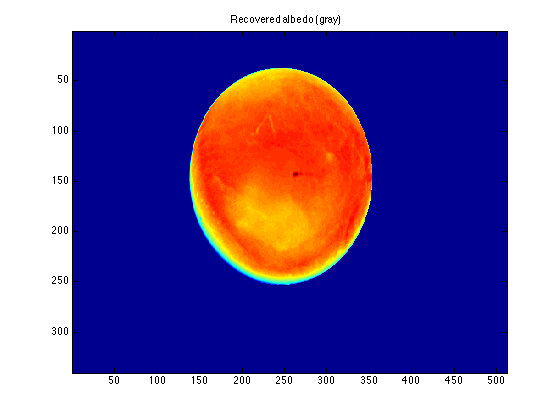
\includegraphics[width=\textwidth]{results/gray/gray_rec_a}
    \end{subfigure}
    ~
    \begin{subfigure}{0.3\textwidth}
        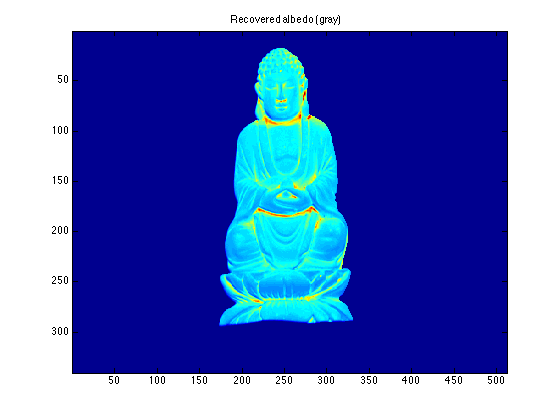
\includegraphics[width=\textwidth]{results/buddha/buddha_rec_a}
    \end{subfigure}
    ~
    \begin{subfigure}{0.3\textwidth}
        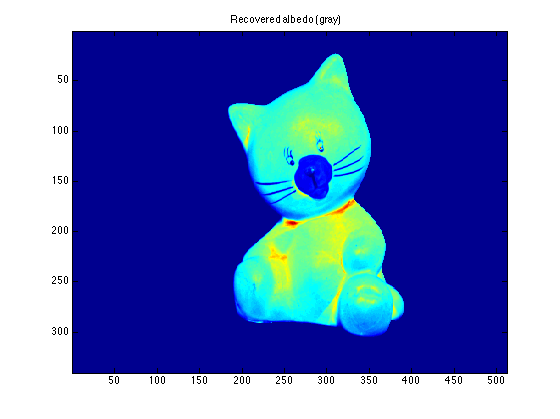
\includegraphics[width=\textwidth]{results/cat/cat_rec_a}
    \end{subfigure}
    
     \begin{subfigure}{0.3\textwidth}
        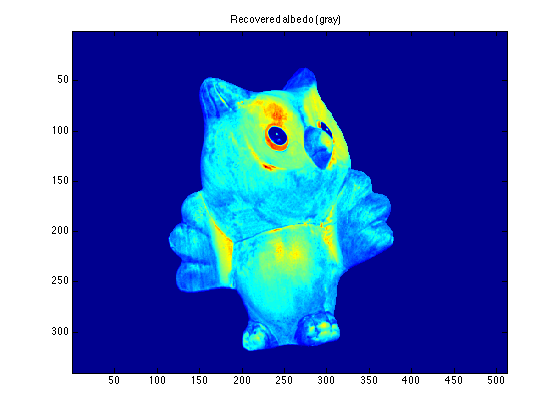
\includegraphics[width=\textwidth]{results/owl/owl_rec_a}
    \end{subfigure}
    ~
    \begin{subfigure}{0.3\textwidth}
        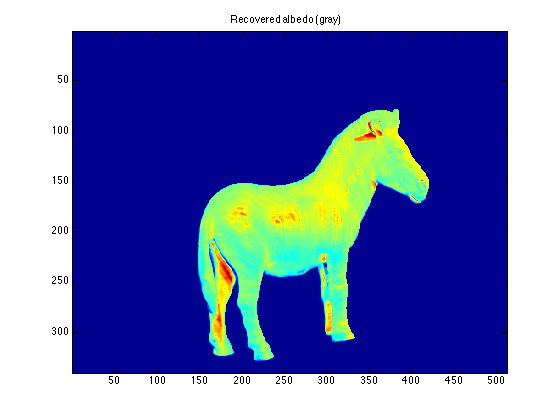
\includegraphics[width=\textwidth]{results/horse/horse_rec_a}
    \end{subfigure}
    ~
    \begin{subfigure}{0.3\textwidth}
        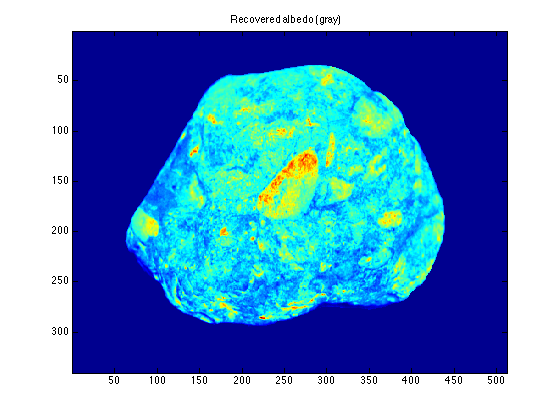
\includegraphics[width=\textwidth]{results/rock/rock_rec_a}
    \end{subfigure}
    \caption{Visualization of the recovered grayscale albedo (luminance) for each dataset}
    \label{fig:rec_albedo}       
\end{figure}

\begin{figure}[h!]
    \centering
    \begin{subfigure}{0.3\textwidth}
        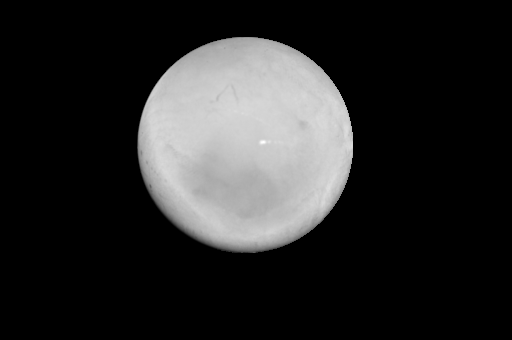
\includegraphics[width=\textwidth]{results/gray/gray_a_lu}
    \end{subfigure}
    ~
    \begin{subfigure}{0.3\textwidth}
        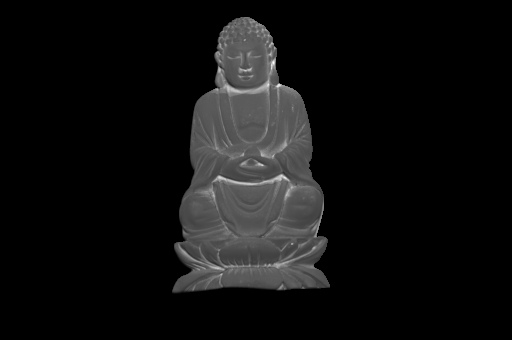
\includegraphics[width=\textwidth]{results/buddha/buddha_a_lu}
    \end{subfigure}
    ~
    \begin{subfigure}{0.3\textwidth}
        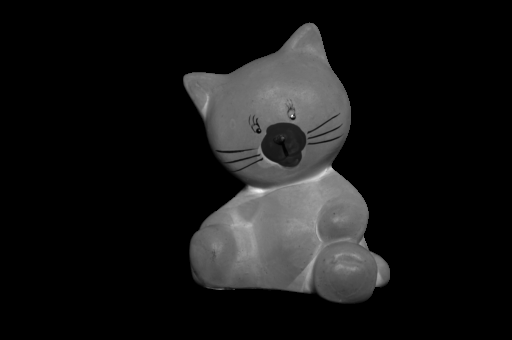
\includegraphics[width=\textwidth]{results/cat/cat_a_lu}
    \end{subfigure}
    
     \begin{subfigure}{0.3\textwidth}
        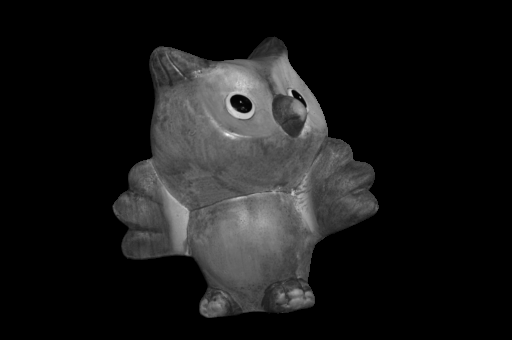
\includegraphics[width=\textwidth]{results/owl/owl_a_lu}
    \end{subfigure}
    ~
    \begin{subfigure}{0.3\textwidth}
        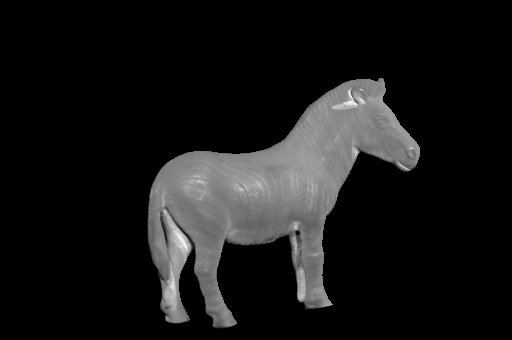
\includegraphics[width=\textwidth]{results/horse/horse_a_lu}
    \end{subfigure}
    ~
    \begin{subfigure}{0.3\textwidth}
        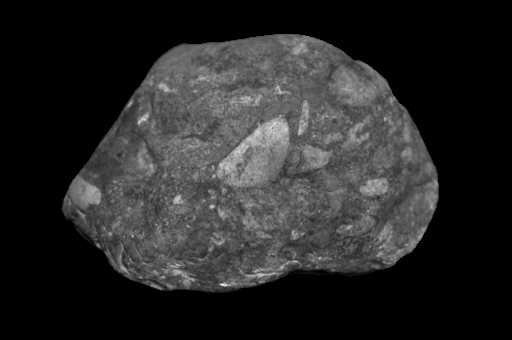
\includegraphics[width=\textwidth]{results/rock/rock_a_lu}
    \end{subfigure}
    \caption{Visualization of the grayscale albedo (luminance) for each dataset}
    \label{fig:albedo_lum}       
\end{figure}


\begin{figure}[h!]
    \centering
    \begin{subfigure}{0.3\textwidth}
        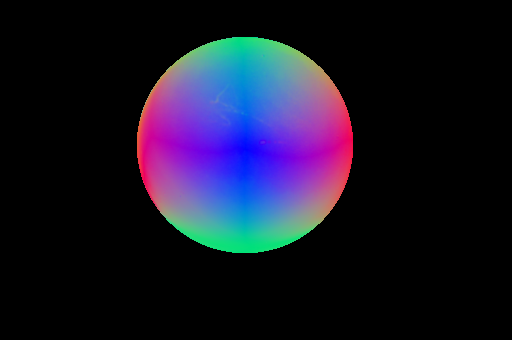
\includegraphics[width=\textwidth]{results/gray/gray_n}
    \end{subfigure}
    ~
    \begin{subfigure}{0.3\textwidth}
        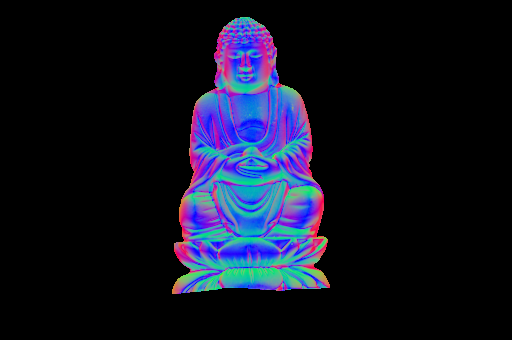
\includegraphics[width=\textwidth]{results/buddha/buddha_n}
    \end{subfigure}
    ~
    \begin{subfigure}{0.3\textwidth}
        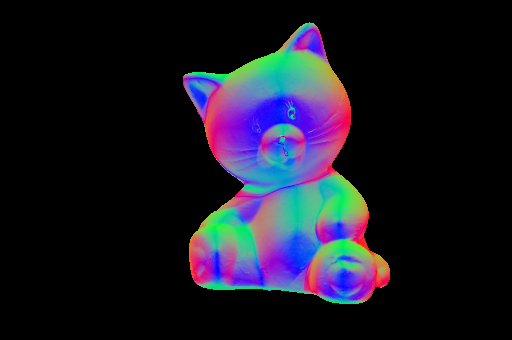
\includegraphics[width=\textwidth]{results/cat/cat_n}
    \end{subfigure}
    
     \begin{subfigure}{0.3\textwidth}
        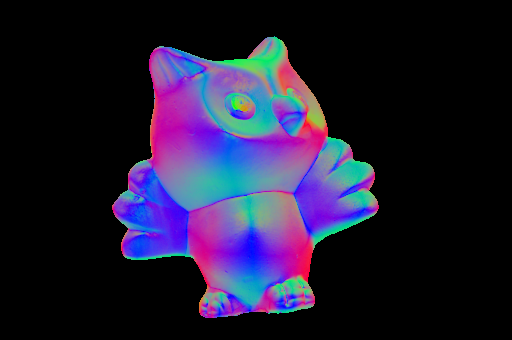
\includegraphics[width=\textwidth]{results/owl/owl_n}
    \end{subfigure}
    ~
    \begin{subfigure}{0.3\textwidth}
        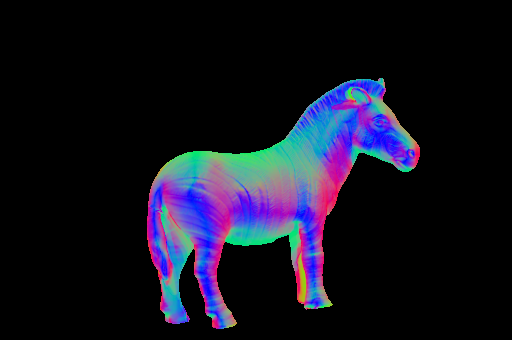
\includegraphics[width=\textwidth]{results/horse/horse_n}
    \end{subfigure}
    ~
    \begin{subfigure}{0.3\textwidth}
        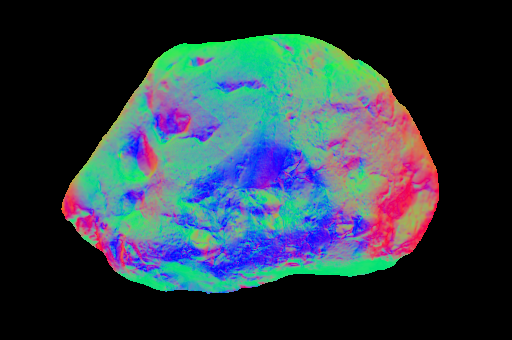
\includegraphics[width=\textwidth]{results/rock/rock_n}
    \end{subfigure}
    \caption{Visualization of the normals for each dataset. Note that each image shows the absolute value applied to each component of each normal vector. The resulting three components are then interpreted as RGB color values. Hence, the x.-axis is pointing to the right, the y-acis is pointing upwards and the z-axis is pointing towards the viewer. }
    \label{fig:normals}       
\end{figure}


\begin{figure}[h!]
    \centering
    \begin{subfigure}{0.45\textwidth}
        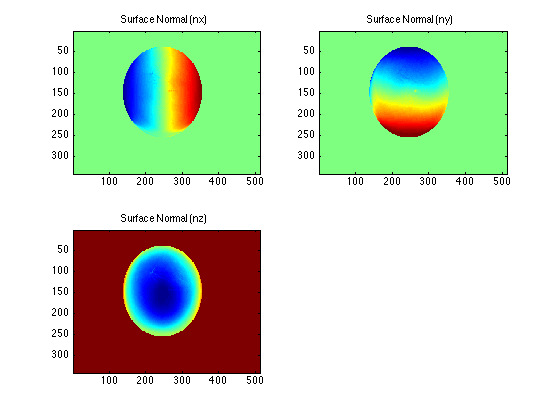
\includegraphics[width=\textwidth]{results/gray/gray_n_xyz}
    \end{subfigure}
    ~
    \begin{subfigure}{0.45\textwidth}
        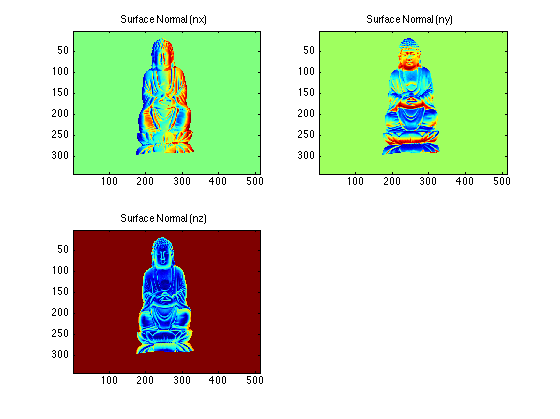
\includegraphics[width=\textwidth]{results/buddha/buddha_n_xyz}
    \end{subfigure}
    
    \begin{subfigure}{0.45\textwidth}
        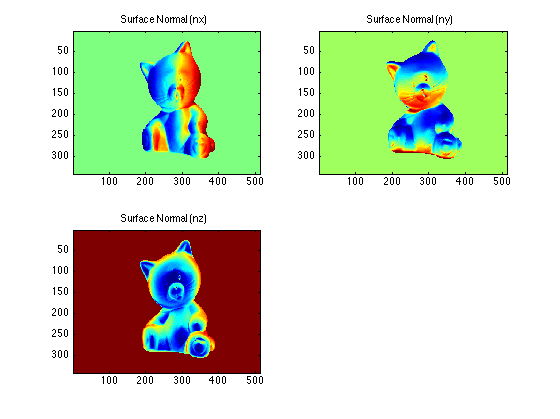
\includegraphics[width=\textwidth]{results/cat/cat_n_xyz}
    \end{subfigure}
    ~
     \begin{subfigure}{0.45\textwidth}
        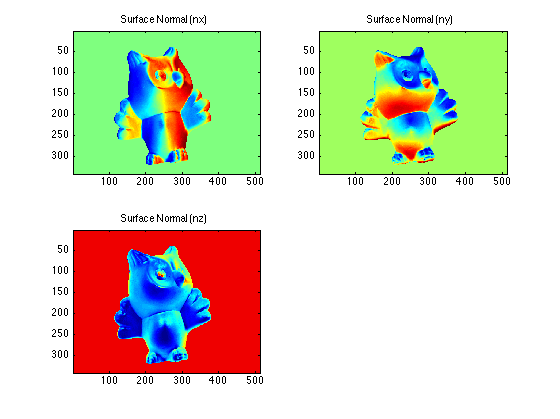
\includegraphics[width=\textwidth]{results/owl/owl_n_xyz}
    \end{subfigure}
    
    \begin{subfigure}{0.45\textwidth}
        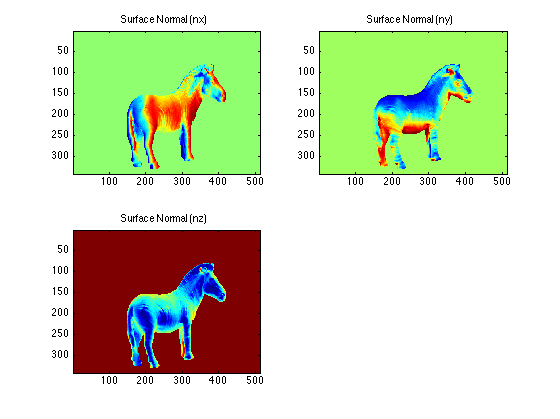
\includegraphics[width=\textwidth]{results/horse/horse_n_xyz}
    \end{subfigure}
    ~
    \begin{subfigure}{0.45\textwidth}
        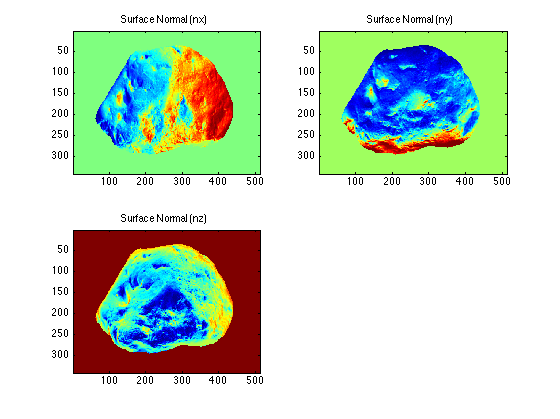
\includegraphics[width=\textwidth]{results/rock/rock_n_xyz}
    \end{subfigure}
    
    \caption{Visualization of the of the three normal components (x,y,z direction) for each dataset.} 
    \label{fig:normals_xyz}       
\end{figure}


\begin{figure}[h!]
    \centering
    \begin{subfigure}{0.3\textwidth}
        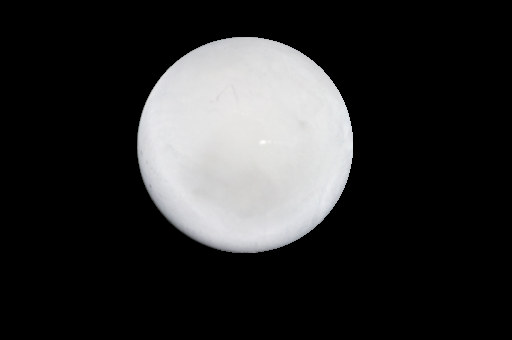
\includegraphics[width=\textwidth]{results/gray/gray_a_rgb}
    \end{subfigure}
    ~
    \begin{subfigure}{0.3\textwidth}
        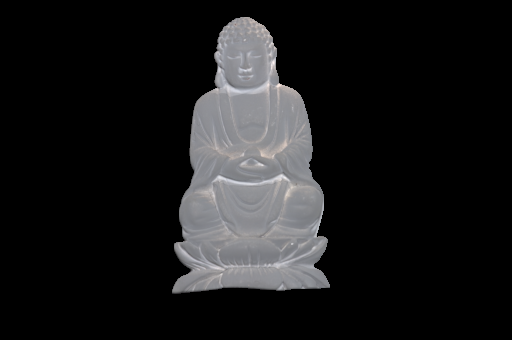
\includegraphics[width=\textwidth]{results/buddha/buddha_a_rgb}
    \end{subfigure}
    ~
    \begin{subfigure}{0.3\textwidth}
        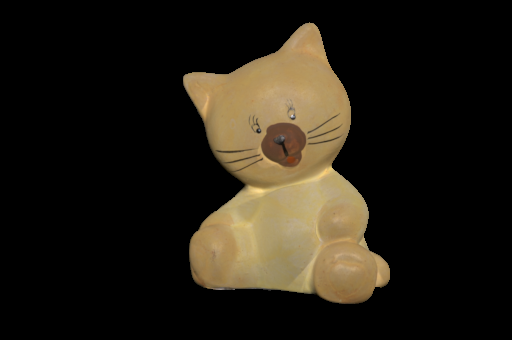
\includegraphics[width=\textwidth]{results/cat/cat_a_rgb}
    \end{subfigure}
    
     \begin{subfigure}{0.3\textwidth}
        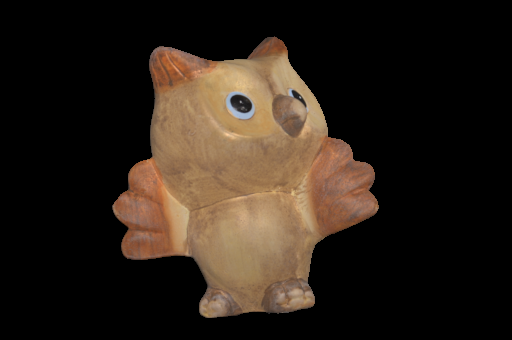
\includegraphics[width=\textwidth]{results/owl/owl_a_rgb}
    \end{subfigure}
    ~
    \begin{subfigure}{0.3\textwidth}
        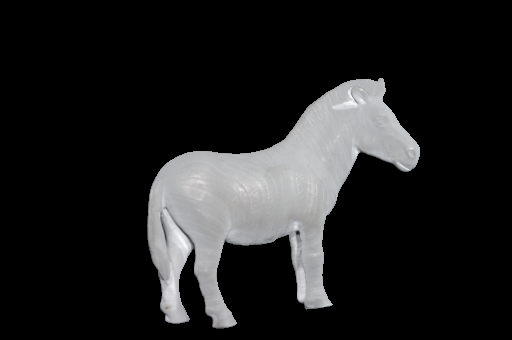
\includegraphics[width=\textwidth]{results/horse/horse_a_rgb}
    \end{subfigure}
    ~
    \begin{subfigure}{0.3\textwidth}
        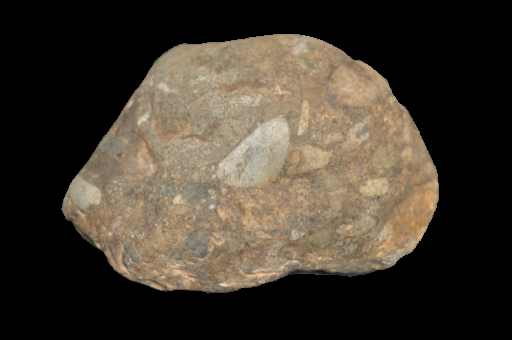
\includegraphics[width=\textwidth]{results/rock/rock_a_rgb}
    \end{subfigure}
    \caption{Visualization of the RGB albedo map for each dataset.}
    \label{fig:albedo_rgb}       
\end{figure}





\paragraph{3. Surface Fitting (35 points)}

In this section you should: 

\begin{itemize}
\item Describe the algorithm you used for calculating the depth map given the normals you calculated before.
\item Display the image of the depth map (in colour or grayscale) for each dataset, where higher intensity values indicate points closer to the camera.
\item Describe, in no more than a few paragraphs, your assessment of when the technique works well, and when there are failures. When the technique fails to produce nice results, please explain as best as you can what the likely causes of the problems are.
\end{itemize}


\textbf{Goal}: Express the depth of a surface S as a function of a surface normal. \\
A surface $S$ in $\mathbb{R}^3$ can be defined by a perametrization 

\begin{equation}
    S(x,y) = (x,y,z(x,y))
\end{equation}

Where $z(x,y)$ depicts the height field value at the point $(x,y)$. For any point on such a paramterized surface $S$ we can span a tangent plane using its tangent vectors at that point.

\begin{align}
    t_x &= \frac{\partial S}{\partial x}(x,y) = (1,0,z_x)^T \nonumber \\
    t_y &= \frac{\partial S}{\partial y}(x,y) = (0,1,z_y)^T
\label{eq:tangent_plane_vectors}
\end{align}

Where $z_x$ denotes the partial derivate of $z$ along the $x$-axis and $z_y$ the partial derivative along the $y$-axis respectively. The tangent plane spanned by those tangent vectors at a point $(x,y)$ from equation $\ref{eq:tangent_plane_vectors}$ have the following normal vector:

\begin{equation}
    \textbf{n}(x,y) = \frac{t_x(x,y) \times t_y(x,y)}{|| t_x(x,y) \times t_y(x,y)||}
\label{eq:tan_plane_normal}
\end{equation}

Using a finite difference scheme we can compute numerically the derivatives of the $z$ component used in equation $\ref{eq:tangent_plane_vectors}$. Finite differences origin from a taylor series approximation by using the first order terms. We get the following approximations for the derivatives of $z$ along the x-and y-axis:

\begin{align}
    z_x(x,y) &= z(x+1,y) - z(x,y) \nonumber \\
    z_y(x,y) &= z(x,y+1) - z(x,y)
\label{eq:fin_diff_approx}
\end{align}

Equation $\ref{eq:fin_diff_approx}$ allows us to solve for the tangent- and normal vectors defined as in equation $\ref{eq:tangent_plane_vectors}$ and equation $\ref{eq:tan_plane_normal}$ respectively. \\

Since every normal vector $\textbf{n}$ is perpendicular to its tangent vectors $t_x$ and $t_y$, i.e.

\begin{align}
    \textbf{n} \cdot t_x &= 0 \nonumber \\
    \textbf{n} \cdot t_y &= 0
\label{eq:gen_constraint_tangents}
\end{align}

we can use this equation $\ref{eq:gen_constraint_tangents}$ as constraint for our tangent vectors:

\begin{align}
    \textbf{n}(x,y) \cdot t_x(x,y &= 0 \nonumber \\
    \textbf{n}(x,y) \cdot t_y(x,y) &= 0
\label{eq:gen_constraint_tangents}
\end{align}

For every point $(x,y)$ on the surface $S$. Applying $d$

\begin{align}
    \left(
        \begin{array}{c}
            1 \\
            0 \\
            z(x+1,y)-z(x,y)
        \end{array}
    \right) 
    \cdot 
    \left(
        \begin{array}{c}
            0 \\
            1 \\
            z(x,y+1)-z(x,y)
        \end{array}
    \right) &= 0 \nonumber \\
        \left(
        \begin{array}{c}
            0 \\
            1 \\
            z(x,y+1)-z(x,y)
        \end{array}
    \right) 
    \cdot 
    \left(
        \begin{array}{c}
            0 \\
            1 \\
            z(x,y+1)-z(x,y)
        \end{array}
    \right) &= 0 
\label{eq:gen_constraint_tangents_ref1}
\end{align}


    
    


\paragraph{Failure cases}
\begin{itemize}
    \item If the material does not exhibit specular hightlights, the method will fail. Actually, materials are assumed to reflect light as a lambertain material does.
    \item surface must be sufficiently smooth. Objects with many sharp edges will produce bad results.
    \item Inter reflection is not taken care of.
    \item Shadows are an issue case, since this method does not take care of self-occlusion.
\end{itemize}



\begin{figure}[h!]
    \centering
    \begin{subfigure}{0.3\textwidth}
        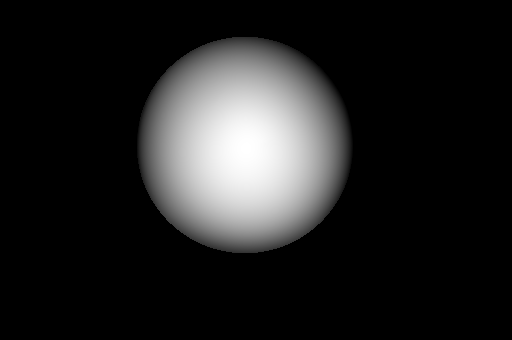
\includegraphics[width=\textwidth]{results/gray/gray_depthmap}
    \end{subfigure}
    ~
    \begin{subfigure}{0.3\textwidth}
        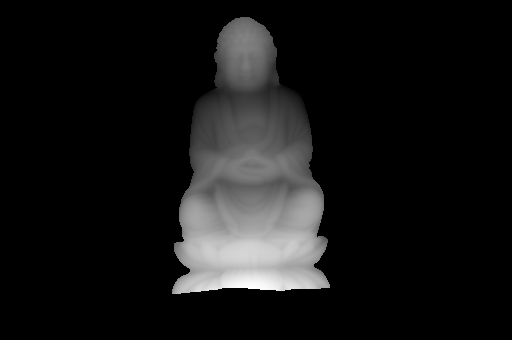
\includegraphics[width=\textwidth]{results/buddha/buddha_depthmap}
    \end{subfigure}
    ~
    \begin{subfigure}{0.3\textwidth}
        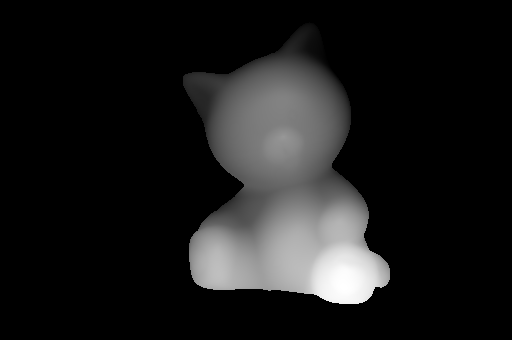
\includegraphics[width=\textwidth]{results/cat/cat_depthmap}
    \end{subfigure}
    
     \begin{subfigure}{0.3\textwidth}
        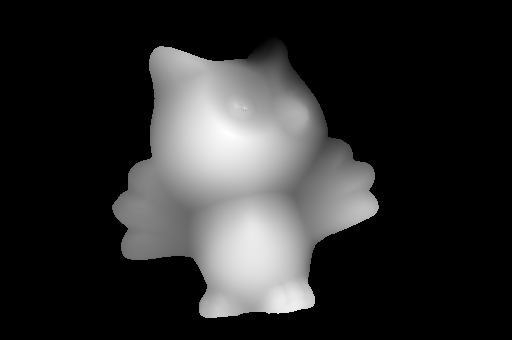
\includegraphics[width=\textwidth]{results/owl/owl_depthmap}
    \end{subfigure}
    ~
    \begin{subfigure}{0.3\textwidth}
        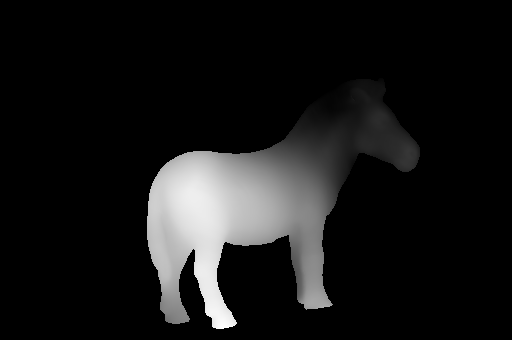
\includegraphics[width=\textwidth]{results/horse/horse_depthmap}
    \end{subfigure}
    ~
    \begin{subfigure}{0.3\textwidth}
        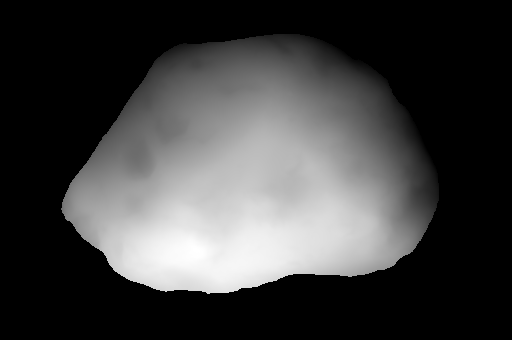
\includegraphics[width=\textwidth]{results/rock/rock_depthmap}
    \end{subfigure}
    \caption{Visualization of the depth map for each dataset. The brighter a pixel looks, the closer it is located to the camera.}
    \label{fig:depthmap}       
\end{figure}




 \end{document}